% !TeX spellcheck = en_GB
% !TeX root = Report.tex
\phantomsection
\addcontentsline{toc}{subsection}{Case 3 - 4G Mobile Broadband}
\subsect{Case 3 - 4G Mobile Broadband}


%Why the wireless spectrum must be controlled and governed. 
The radio spectrum is considered a state's national renewable resource.
Since the first wireless broadcast in 1897, wireless communications has grown hugely. % \citeneeded{}.
The rise of the semiconductor unlocked higher radio frequencies, enabling the use of more of the spectrum.
The current radio spectrum spans from $3kHz$ to $300 GHz$. 
A simplified diagram of the radio spectrum in the United Kingdom can be seen in Figure~\ref{c3:ukspectrum}, but in reality, it is much more complex \cite{roke:ukspectrum}.

\begin{figure}
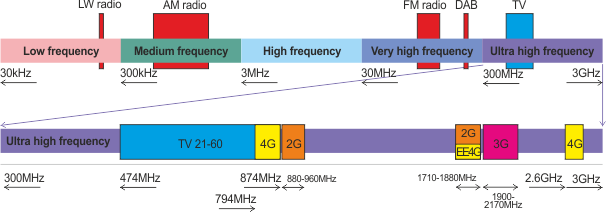
\includegraphics[width=\textwidth]{Figures/radiospectrum.png}
\caption{A simplified diagram of the UK Radio Spectrum from \cite{ukfreetv}}
\label{c3:ukspectrum}
\end{figure}

The allocation of radio spectrum must be managed to avoid interference. 
A large number of devices rely on wireless communications, from GPS, mobile phones and even car keys.
Signal interference between devices is considered an issue with wireless communications \cite{GPS}. 
Therefore the allocation of radio frequencies is now done by a governing board, Ofcom \cite{ofcom:whatis}.
By correctly managing the spectrum, money can be made an innovation can be encouraged.

The switch off of analogue TV in the UK freed up a large amount of the spectrum \cite{ofcom:tv}.
This has since been reallocated to be used for 4G Mobile Broadband.
The allocations can be seen in Figure~\ref{c3:ukspectrum}.

The allocation is done by a spectrum auction.
Companies each put bids in for use of the spectrum. 
If a company wins the auction, this allows them to transmit using the allocated frequencies. 
The auction for the 4G spectrums raised \pounds 2,340 million. 

A well-designed auction is key. 
Competition must be allowed, as a monopoly over a spectrum, and therefore a technology, causing a lack of innovation and high prices. 
However, the companies must be well equipped to be able to fulfil the ability to provide the service.
In the 4G auction, there were two main frequency bands available - the low frequency $800MHz$ band and a high frequency $2.6GHz$ band. 
The compromise made here is between coverage and speed: the higher frequency can support a higher density of traffic with a higher speed, but the lower frequency is more suitable to rural areas and provides better signal to the users.

The results of the auction saw Vodafone, Three and O2 have a portion of the low frequency. 
Vodafone and EE were awarded a part of the high frequency.
EE already owned the middle 4G frequency which is leased to Three. 
This should generate healthy competition in not only the high speed market. 

However, spectral auctions can cause issues.
The 3G spectrum was originally auctioned in 2000. 
The money raised fell short of the \pounds 3,500 million by \pounds 1,000 million \cite{telecom}.
In Europe, companies overpaid for the 3G licenses and ran up huge debts.
This, combined with home broadband expectations, was a huge overestimation of the data demand and caused the Telecoms Crash in 2001 \cite{telecom:crash}.
It is thought that the 3G spectral auctions contributed to this crash.

In conclusion, governance is needed in the mobile and wireless communication markets for two main reasons.
Firstly, the spectrum must be managed to ensure that the technologies are not subject to accidental interference, causing the technology to fail. 
Secondly, the competition must be managed to keep costs down and encourage innovation between the rivalling companies. 


